% \subsection{Flatsat}

% Most of the tests were performed on Flatsat (an abbreviation from Flat Satellite), an electronic test bench, which consist of mix of flight models, engineering models of the instruments and Electrical Ground Support Equipment (EGSE). EGSE are the test instruments and/or mocks (fake) instruments, which allow testing without the need for actual hardware.

% PW-Sat2 Flatsat was integrated in Space Research Centre in Warsaw. Flatsat is shown in the figure \ref{TODO}.

% \subsubsection{Flatsat Ground Station mock}
% To perform the communication tests a Ground Station mock was created of flatsat. It was built using to Software-Defined Radios: one, as downlink receiver, same as to be installed in the Ground Station (Funcube Pro+), and the second (PlutoSDR) to generate uplink signals. Use of SDR instead of analogue radio transceiver greatly simplified the tests performed. Ground station mock is shown in the figure \ref{TODO}. 




\chapter{Space segment}
Space segment is a part of the satellite communication system that resides on the satellite itself. It is divided into two main parts: communication subsystem (COMM) and antennas (ANTs) connected with two coaxial cables.

Space segment is critical in system operation and reliability - there is no possibility to carry out any repairs, perform maintenance or adjustment once on orbit. It is exposed to the space environment - wide temperature range, thermal cycling, cosmic radiation and vacuum.

Because of the mentioned requirements it was decided to choose commercially available and flight-proven CubeSat components to increase the overall reliability of the system.

% -----------------------------------------------------------------------------------------------------------
% -----------------------------------------------------------------------------------------------------------
% -----------------------------------------------------------------------------------------------------------

\section{Spacecraft communication transceiver}
\label{section:comm_design}
CubeSat design specification \cite{cubesat_spec}, with which PW-Sat2 is compliant, defines common PC/104 connector, which is the main data bus for all satellite subsystems. On the connector, two \iic and two CAN buses are defined and most of the components are compatible to each other. However, due to the lack of CAN interface on On-Board Computer (CubeComputer from CubeSpace \cite{cubespace_website}) radio should use \iic communication bus.

When the subsystem was ordered (in year \si{2014}), the choice of available products was very limited, and the only radio which was compliant with above mentioned requirements was \texttt{ISIS VHF uplink/UHF downlink Full Duplex Transceiver}. Its view and block diagram is shown in the figure \ref{ISIS_TRXvU}

\begin{figure*}
   \centering
\begin{tabular}{cc}
        \includegraphics[width=0.3\paperwidth]{img/4/ISIS-radio-UHF-VHF-min.png}
    & 
        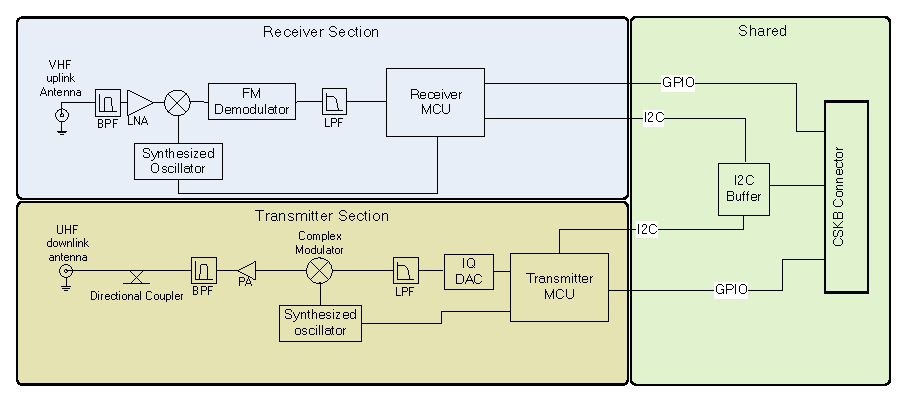
\includegraphics[width=0.4\paperwidth]{img/4/ISIS_TRXvU_block_diagram.eps}
\end{tabular}
\label{ISIS_TRXvU}
\caption{ISIS VHF uplink/UHF downlink Full Duplex Transceiver. Source: \cite{isis_trxvu}}
\end{figure*}

Basic characteristics: \\
\begin{tabular}{c|c}
     \textbf{downlink} & \textbf{uplink} \\ \hline
     \multicolumn{2}{c}{dual-\iic communication standard} \\
     \multicolumn{2}{c}{AX.25 frame format} \\
     \si{430}-\SI{450}{\MHz} frequency range & \si{140}-\SI{150}{\MHz} frequency range \\
     \SI{0.5}{\watt} downlink power & \SI{-98}{\dBm} sensitivity for \si{10^-5}~BER \\
     \si{1.2} - \SI{9.6}{\kilo\bit / \second} bitrate & \SI{1.2}{\kilo\bit / \second} bitrate \\ 
     BPSK modulation with G3RUH scrambling & FM-modulated AFSK \\ 
\end{tabular}

Transceiver was tested separately for its uplink and downlink capabilities. Tests are critical to make sure that radio parameters are maintained in the system, and to verify manufacturers' data.

\subsection{Uplink measurements}
The most important parameter of the radio receiver is the sensitivity. Blocking immunity (intermodulation), is not critical, as the system is remote from most of the external strong radio signals.

\subsubsection{Sensitivity}
Sensitivity was measured by the setup shown in the figure \ref{TODO}. Test procedure:
\begin{itemize}
    \item measuring output power of PlutoSDR using spectrum analyzer with wide RBW filter (\SI{1}{\MHz})
    \item increasing attenuation up to the point when PER is noticeable (\SI{1}{\percent})
    \item calculating signal input power
\end{itemize}

The result of this test was the sensitivity of TODO.

\subsubsection{Doppler}
Doppler effect is caused when fast-moving object is emitting/receiving radio waves. For uplink frequency (VHF band) Doppler effect influence can shift frequency up to about \SI{5}{\kHz}. The receiver bandwidth should be measured to estimate allowable frequency inaccuracies.

Test setup is the same as in previous setup, shown in the figure \ref{TODO}. During the test the PER was measured for a range of frequency shift from center. The result is shown in the chart \ref{TODO}.

\subsection{Downlink measurements}
Downlink parameters of the radio module were also measured. An important parameter is the output power and the spectrum of the signal.

\subsubsection{Output power}
Output power was measured using spectrum analyser with wide resolution bandswidth (\SI{1}{\MHz}). Output power was measured to be \SI{27}{\dBm}. TODO

\subsubsection{Spectrum}




% -----------------------------------------------------------------------------------------------------------
% -----------------------------------------------------------------------------------------------------------
% -----------------------------------------------------------------------------------------------------------



\section{Spacecraft Antennas}
Because of the selected radio system, two antennas has to be installed - one for uplink (VHF) and one for downlink (UHF). Antennas should be omnidirectional, as PW-Sat2 does not have an nadir-pointing capability and random tumbling during operation is assumed.

Self-made dipole antenna was considered at the design stage, but due to mechanical and time constraints, satellite antenna was decided to be bought as well. Innovative Solutions In Space company sells antenna with with the transceiver as CubeSat communication Kit \texttt{CubeSat dipole antenna system}. Both elements are compatibile and the whole system (transceiver + antenna) is tuned for specific communication frequency and mounting option.

This system is deployable by the command from the on-board computer. Thermal knife (resistor) is heated up and thermal link is burnt, resulting is antenna deploy by the spring action. Antenna is shown in the figure \ref{ISIS_antenna}.

\begin{figure*}
   \centering
\begin{tabular}{cc}
        \includegraphics[width=0.3\paperwidth]{img/4/isis_antenna_stowed.jpg}
    & 
        \includegraphics[width=0.45\paperwidth]{img/4/CubeSat-antenna-dipole-configuration.png}    
\end{tabular}
\label{ISIS_antenna}
\caption{ISIS CubeSat dipole antenna system in stowed and deployed position. Source: \cite{isis_dipole_antenna}}
\end{figure*}


\subsection{Measurements}
After deployment on the orbit, antennas have to deploy. During the test campaign antenna deployment procedure was executed three times. Deployed antennas are shown in the figure \ref{TODO}.

Reflected power from antenna is measured by the radio module during radio frame transmission. Correct antenna deployment can be assured by using the telemetry and comparing the reflected power with measured during the ground test campain. 
Reflected and forward power chart captured during second antenna opening are shown in the figure \ref{TODO}.

% -----------------------------------------------------------------------------------------------------------
% -----------------------------------------------------------------------------------------------------------
% -----------------------------------------------------------------------------------------------------------

% \subsubsection{Deployable elements influence on the antenna pattern}
% TODO

% On-board PW-Sat2 are two main deployables: solar panels and deorbitation sail.

% During design stage, influence of the solar panels was discussed with antenna manufacturer - the outcome was to place longed dipoles (VHF) along the solar panels, and shorter ones orthogonally to it, as shown in the figure \ref{???}

% % TODO: zdjęcie z otwartymi panelami i antenami

% The influence of the deorbit sail was also simulated during Critical Design stage.

% Deorbitation sail is made by very thin (\SI{5}{\micro\meter}) mylar foil with aluminium coating. Using % TODO
% simulation tool, it was shown that the sail will increase directivity of the cubesat antennas, acting as a reflector.
% % TODO: jakieś zdjęcie z symulacji, wynik o ile dB się pogorszyło


